% Подписи колонтитула
\newcommand{\colontitulAutors}{astronom\_v\_cube}
\newcommand{\colontitulYear}{2022}
\newcommand{\colontitulEducationalSubject}{Теория колебаний}
\newcommand{\colontitulTeacher}{Некоркин В.И.}

%Настройки шаблона
\documentclass[10pt,landscape,a4paper]{article}
\usepackage[utf8]{inputenc}
\usepackage[english, russian]{babel}
\usepackage[T1,T2A]{fontenc}  
\usepackage{upgreek} % прямые греческие ради русской традиции
\usepackage{tikz}
\usetikzlibrary{shapes,positioning,arrows,fit,calc,graphs,graphs.standard}
%\usepackage[nosf]{kpfonts}
%\usepackage[t1]{sourcesanspro}
\usepackage{multicol}
\usepackage{wrapfig}
\usepackage[top=6mm,bottom=8mm,left=4mm,right=4mm]{geometry}
\usepackage[framemethod=tikz]{mdframed}
\usepackage{microtype}
\usepackage{pdfpages}
\usepackage{amsthm,amsmath,amscd}   % Математические дополнения от AMS
\usepackage{amsfonts,amssymb}       % Математические дополнения от AMS
\usepackage{mathtools}              % Добавляет окружение multlined
\usepackage{xfrac}                  % Красивые дроби
\usepackage{physics}

\usepackage{fancyhdr} % колонтитулы

%некоторые математические команды
\newcommand{\Div}{\operatorname{div}}
\newcommand{\Grad}{\operatorname{grad}}

\let\bar\overline

\definecolor{myblue}{cmyk}{1,.72,0,.38}

\def\firstcircle{(0,0) circle (1.5cm)}
\def\secondcircle{(0:2cm) circle (1.5cm)}

\colorlet{circle edge}{myblue}
\colorlet{circle area}{myblue!5}

\tikzset{filled/.style={fill=circle area, draw=circle edge, thick},
	outline/.style={draw=circle edge, thick}}

\pgfdeclarelayer{background}
\pgfsetlayers{background,main}

%\everymath\expandafter{\the\everymath \color{myblue}}
\everydisplay\expandafter{\the\everydisplay \color{myblue}}

\renewcommand{\baselinestretch}{.8}
\pagestyle{empty}

\global\mdfdefinestyle{header}{%
	linecolor=gray,linewidth=1pt,%
	leftmargin=0mm,rightmargin=0mm,skipbelow=0mm,skipabove=0mm,
}

\makeatletter % Author: ttps://tex.stackexchange.com/questions/218587/how-to-set-one-header-for-each-page-using-multicols
\renewcommand{\section}{\@startsection{section}{1}{0mm}%
	{.2ex}%
	{.2ex}%x
	{\color{myblue}\sffamily\small\bfseries}}
\renewcommand{\subsection}{\@startsection{subsection}{1}{0mm}%
	{.2ex}%
	{.2ex}%x
	{\sffamily\bfseries}}

\makeatother
\setlength{\parindent}{0pt}

%колонтитулы
\pagestyle{fancy}
\fancyhf{}
\setlength{\headheight}{40pt}
\setlength{\headsep}{4pt}
\renewcommand{\headrulewidth}{1pt}
\fancyhead[L]{\textcopyright~\colontitulAutors}
\fancyhead[C]{Программа минимум по курсу <<\colontitulEducationalSubject>> \colontitulYear г}
\fancyhead[R]{Преподаватель:~\colontitulTeacher}

\begin{document}
	\small
	\begin{multicols*}{2}
		\textbf{Базовые понятия}\\
		Фазовое пространство — совокупность всех начальных точек $X$ или всех возможных состояний системы. Фазовая траектория — кривая в фазовом пространстве, составленная из точек, представляющих состояние динамической системы в последовательные моменты времени в течение всего времени эволюции.\\
		Эволюция системы соответствует движению изображающей точки у фазовой плоскости вдоль траектории $\text{Г} = \bigcup_t G^t X_0$. Для динамической системы с непрерывным временем траектории— непрерывные кривые для динамической системы с дискретным временем, траектория— дискретные, подмножество фазовой плоскости.\\
		Динамическая система с непрерывным временем задается системой дифференциальных уравнений $\dot{x} = F(x)$. Она позволяет найти состояние в любой момент времени по начальному состоянию.
		Если правая часть явно от времени не зависит, то динамическая система -  автономная, иначе - не автономная.\\
		Динамическая система с дискретным временем: $x(n+1) = F(x(n))$.
		
		\section{Определение динамической системы}
		Рассмотрим систему, состояние которой определяется вектором $x(t)\in R^n$.
		Предположим, что эволюция системы определяется одно-параметрическим семейством операторов $G^t, t \in R$ или $t \in Z$, таких, что состояние системы в момент $t$: $x(t, x_0 = G^t x_0)$
		где $x_0$ – начальное состояние (начальная точка). Предположим также, что эволюционные операторы удовлетворяют двум следующим свойствам,
		отражающим детерминистический характер описываемых процессов.\\
		Первое свойство: $G^0$ – тождественный оператор, т.е. $x(0,x_0 ) = x_0$, для любых $x_0$. Это свойство означает, что состояние системы не может изменяться самопроизвольно.\\
		Второе свойство эволюционных операторов имеет вид: $x(t_1+t_2, x_0) = x(t_1, x(t_2, x_0)) = x(t_2, x(t_1, x_0))$ Согласно ему, система приходит в одно и то же финальное состояние независимо от того, достигается ли оно за один временной интервал $t_1+t_2$, или за
		несколько последовательных интервалов $t_1$ и $t_2$, суммарно равных $t_1+t_2$.\\
		Совокупность всех начальных точек $Х$ или всех возможных состояний
		системы называется фазовым пространством, а пара $(X,{G^t})$, где семейство эволюционных операторов удовлетворяют условиям выше – динамической системой (ДС).\\
		Иначе говоря, динамическая система — объект или процесс, для которого однозначно определено понятие состояния, как совокупности некоторых величин в данный момент времени и задан закон эволюции начального состояния с течением времени. По этому закону можно прогнозировать будущее состояние динамической системы.
		
		\section{Условия грубости динамических систем на плоскости}
		Так как динамические системы изменяются вместе со входящими в них параметрами, но при малости изменений качественные черты поведения сохраняются, вводится свойства грубости. Грубость — устойчивость структуры разбиения фазовой плоскости динамических систем на траектории по отношению к малым изменениям динамической системы.\\
		Для плоскости: пусть есть система:\\
		$\begin{cases}
			\dot{x} = P(x,y) \\
			\dot{y} = Q(x,y)
		\end{cases} $\\
		где $P$ и $Q$ - гладкие функции, система диссипативна.\\
		Система — грубая, если существует число $\delta>0$, что все динамические системы вида:\\
		$\begin{cases}
			\dot{x} = P(x,y) + p(x,y) \\
			\dot{y} = Q(x,y) + q(x,y)
		\end{cases} $\\
		в которых аналитические функции удовлетворяют условию $\left\lvert p(x,y)\right\rvert  + \left\lvert q(x,y)\right\rvert + \left\lvert \dfrac{\partial p}{\partial x}\right\rvert + \left\lvert \dfrac{\partial q}{\partial x}\right\rvert + \left\lvert \dfrac{\partial p}{\partial y}\right\rvert + \left\lvert \dfrac{\partial q}{\partial y}\right\rvert < \delta $, имеют такую же структуру разбиения на положительные полутраектории, что и начальная система.\\
		Переход от одной грубой ДС к другой происходит через негрубую ДС.\\
		ДС на прямой устойчива (структурно грубая), если для всех состоянии равновесия $\lambda_i(\mu)\neq 0$.
		
		\section{Бифуркация состояний равновесия динамических систем на прямой}
		Значение параметра, при котором ДС является негрубой, называется бифуркационным.\\
		Пусть есть динамическая система на прямой общего вида $\dot{x} = F(x, \mu)$. $F(x)$ - взаимооднозначная, обеспечивающая выполнение теорем существования и единственности решений. Тогда состояния равновесия будут определяться как $F(x, \mu) = 0$\\
		$\divideontimes$ Двукратное равновесие: $\dot{x} = \mu \pm x^2$\\
		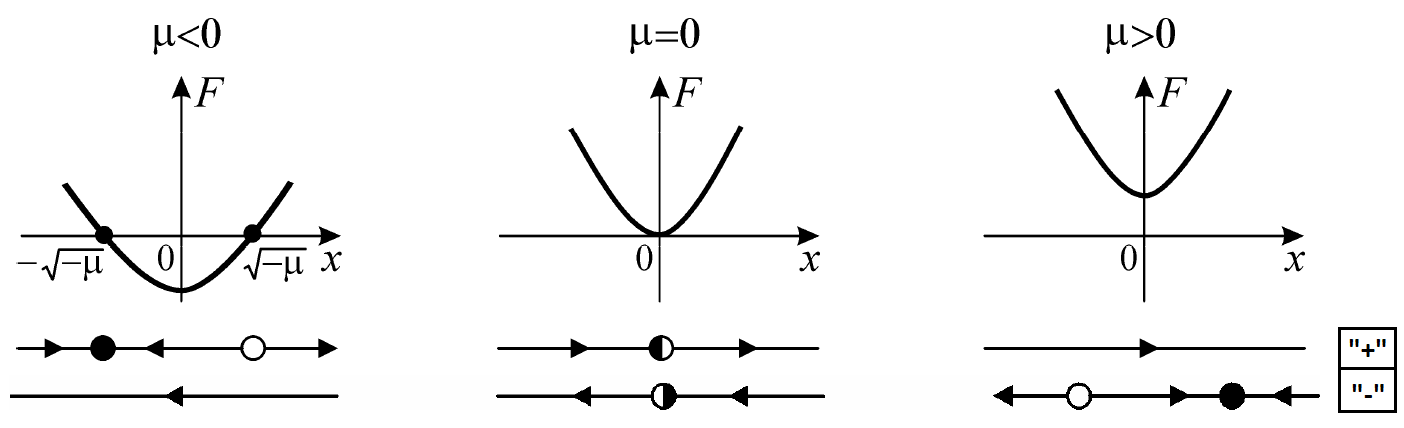
\includegraphics[width=0.75\linewidth]{tk_img/bifurk_1.png}\\
		$\divideontimes$ Транскритическая бифуркация: $\dot{x} = \mu x \pm x^2$\\
		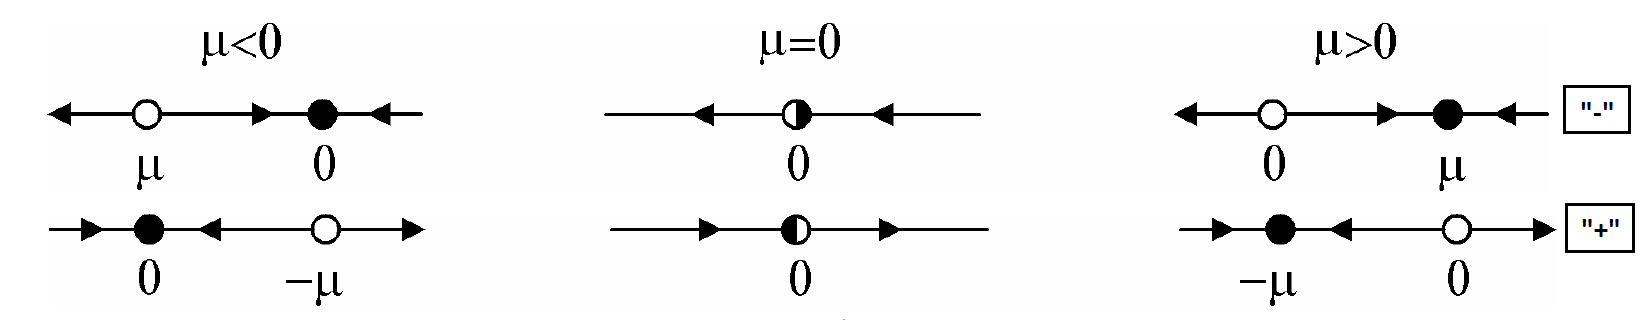
\includegraphics[width=0.75\linewidth]{tk_img/bifurk_2.png}\\
		$\divideontimes$ Трехкратное равновесие: $\dot{x} = \mu x \pm x^3$\\
		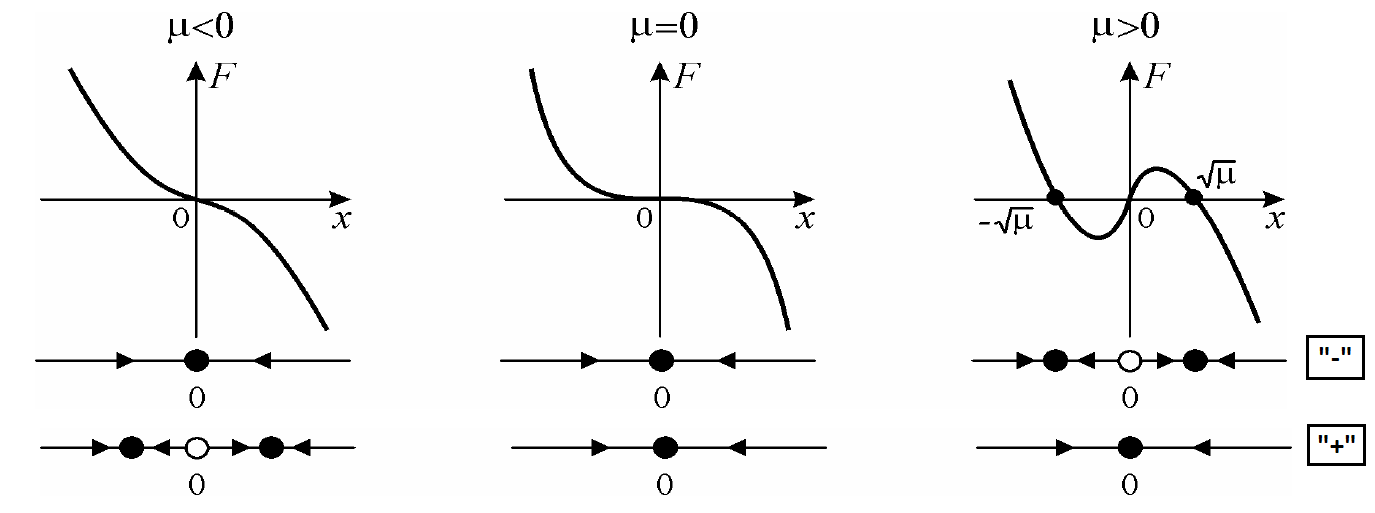
\includegraphics[width=0.75\linewidth]{tk_img/bifurk_3.png}\\
		
		\section{Метод линеаризации определения устойчивости состояний равновесия}
		Рассматриваем систему $n$-ого порядка:$\dot{x} = F(x), x\in R^n, F(x)$ - гладкая вектор-функция. Пусть система имеет состояние равновесия $x = x^*$\\ Введем малое возмущение $\dot{\xi} = F(x^* + \xi)$, разложим правую часть в ряд Тейлора: $\dot{\xi} = A\xi + \dots$, где $A$ - матрица Якоби $m$ с элементами $a_{ik} = \dfrac{\partial F_i}{\partial x_k}|_{x=x^*}$, и отбросим все нелинейные по $\xi$ слагаемые. Этим мы линеаризовали систему.\\
		Решения ищем в виде $\xi = Ce^{\lambda t}$, $C$ - матрица-столбец. Подставив это решение в линеаризованное уравнение мы перейдем к системе линейных однородных уравнений, которая имеет нетривиальное решение, если $det (A-\lambda E) = 0$. Это уравнение эквивалентно $a_0 \lambda ^n + a_1 \lambda ^{n-1} + \dots + a_n = 0$ - характеристическому уравнению. Его корни - характерестические показатели состояния равновесия $x=x^*$\\
		\textbf{1. Все корни имеют отрицательные вещественные части} ($Re \lambda_i < 0$) - состояние равновесия системы асимптотически устойчиво\\
		\textbf{2. Среди корней есть корень с $Re > 0$} - состояние равновесия неустойчиво по Ляпунову\\
		\textbf{3. Среди корней нет значений с $Re > 0$, но есть корень с $Re = 0$} - состояние равновесия может быть как устойчивым, так и неустойчивым
		
		\section{Линейный осциллятор. Основные свойства}
		Осциллятор - простейшая динамическая система с двумерным фазовым портретом\\
		Уравнение ЛО: $\ddot{x} + 2\delta \dot{x} + \omega_0^2 = 0$, \quad $2\delta = \frac{R}{L}, \quad \omega_0^2 = \frac{1}{LC}$\\
		$\delta $ - потери, $\omega_0$ - частота собственных колебаний\\
		\textbf{1. Без потери энергии}\\
		$\begin{cases}
			\dot{x} = y \\
			\dot{y} = -\omega_0^2 x
		\end{cases} $
		\quad \quad $\lambda_{1,2} = \pm i\omega_0$\\
		Состояние равновесия в начале координат - центр\\
		\textbf{Свойства:}\\
		$\divideontimes$ Гармонические колебания происходят с частотой $\omega_0$, амплитудой $A = \sqrt{{x_0}^2} + \dfrac{{y_0}^2}{\omega_0^2}$ и фазой $tg \varphi = \dfrac{\omega_0 x_0}{\omega_0^2}$ ($x_0$ и $y_0$ - в момент $T$)\\
		$\divideontimes$ Колебания изохронны - не зависят от начальных условий\\
		$\divideontimes$ Энергия системы сохраняется\\
		\textbf{2. С потерями энергии ($\delta \neq 0$)}\\
		$\begin{cases}
			\dot{x} = y \\
			\dot{y} = -2\delta y-\omega_0^2 x
		\end{cases} $
		\quad \quad $\lambda^2 + 2\delta \lambda + \omega_0^2 = 0$ - характерестическое ур-е\\
		$\divideontimes$ Затухающий процесс ($\delta > 0, \delta^2 < \omega_0^2$):\\
		$\omega = \sqrt{\omega_0^2 - \delta^2}, \quad \lambda_{1,2} = -\delta \pm i\omega_0$\\
		Состояние равновесия - устойчивый фокус, затухающие колебания с изоклиной - экспонентой\\
		$\divideontimes$ Затухающий апериодический процесс ($\delta > 0, \delta^2 > \omega_0^2$):\\
		$\lambda_{1,2} = -\delta \pm \sqrt{\delta^2 - \omega_0^2}$, состояние равновесия - устойчивый узел\\
		$\divideontimes$ Отрицательное затухание ($\delta<0$): энергия растет во времени, состояние равновесия - неустойчивый фокус при $\delta^2<\omega_0^2$ или неустойчивый узел при $\delta^2\geqslant \omega_0^2$

		\section{Резонанс в линейном осцилляторе}
		Резонанс — неограниченное возрастание амплитуды вынужденных колебаний, когда частота внешней силы близка к собственной частоте, линейного осциллятора.\\
		\textbf{1. Консервативный случай (без потери энергии)}\\
		$W$ - не диссипирует. $a = \dfrac{F_0}{\left\lvert \omega_0^2 - \omega^2\right\rvert }$ - амплитуда вынужденных колебаний переменной x(t).\\
		При резонансе измерение переменных во времени - непереодическое: $x(t) = t\dfrac{F_0}{2\omega_0}sin(\omega_0 t)$\\
		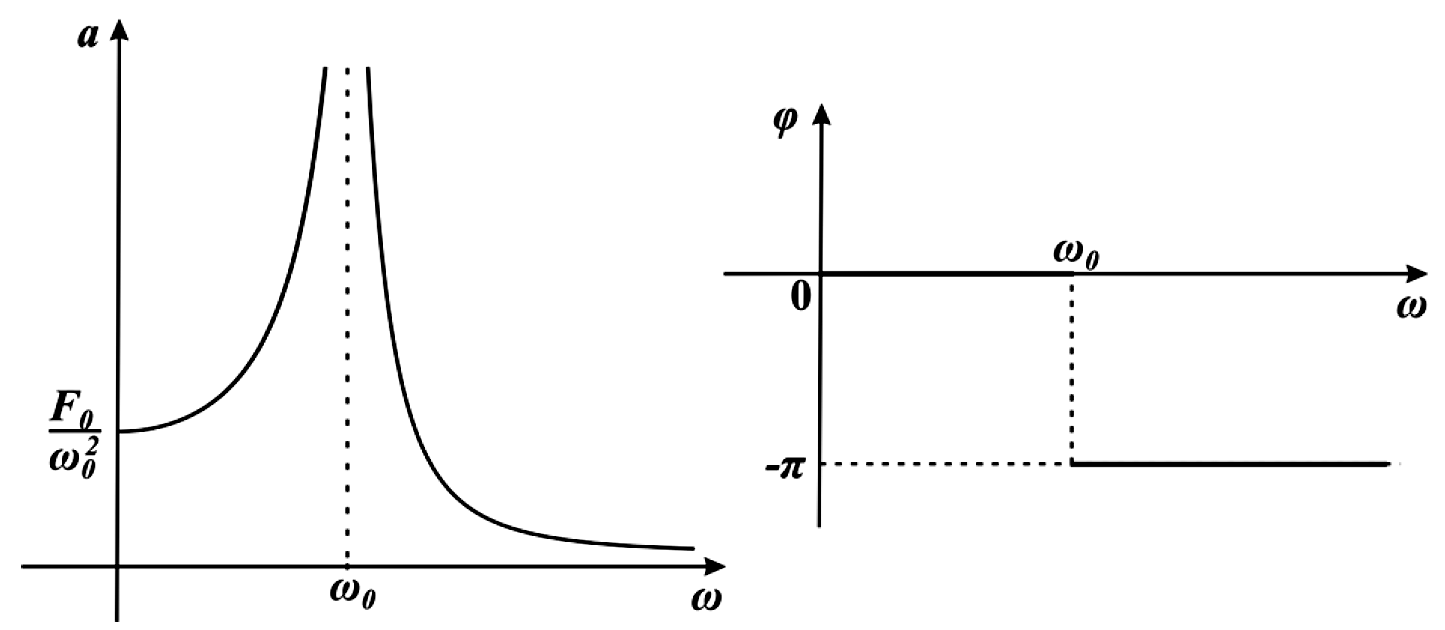
\includegraphics[width=0.6\linewidth]{tk_img/rezonans_1.png}\\
		\textbf{2. Диссипативный случай (с потерями энергии)}\\
		$a_{max}\to \omega_{max}<\omega_0, \quad \omega_{max} = \sqrt{\omega_0^2 - 2\delta^2}, \quad a_{max} = \dfrac{F_0}{2\delta \sqrt{\omega_0^2 - 2\delta^2}}, \quad \delta \uparrow a_{max} \downarrow $\\
		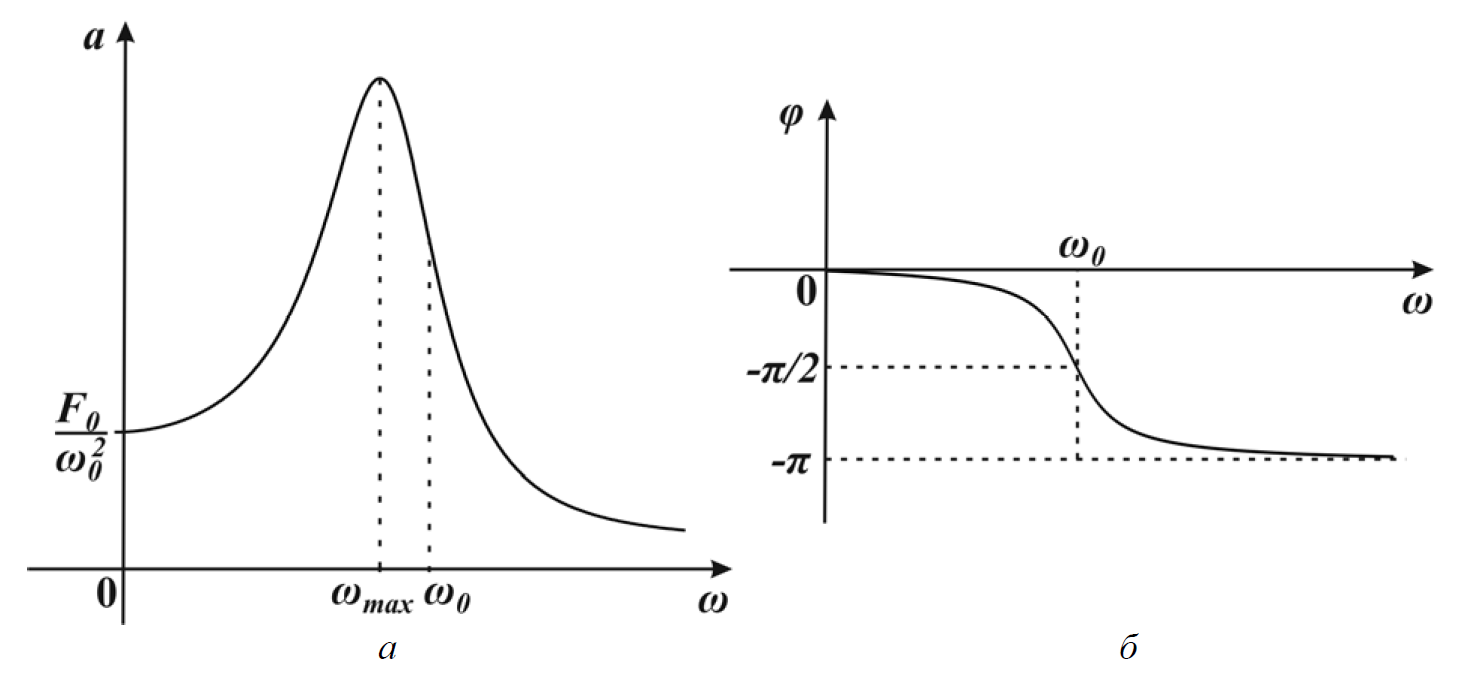
\includegraphics[width=0.6\linewidth]{tk_img/rezonans_2.png}\\
		\textbf{Характеристики резонансных свойств}\\
		Добротность - $Q = \dfrac{\pi}{d} = \dfrac{\omega_0}{2\delta}$\\
		Логарифмический коэффициент затухания - $d = \delta T = \dfrac{2\pi \delta }{\omega}$
		
		\section{Определение предельного цикла. Характеристики}
		Предельный цикл — замкнутая изолированная фазовая траектория. Замкнутая фазовая траектория называется изолированный, если существует достаточно малое кольцеобразная окрестность этой траектории, внутри которой нет других замкнутых траекторий.\\
		Предельному циклу соответствует периодический процесс.\\
		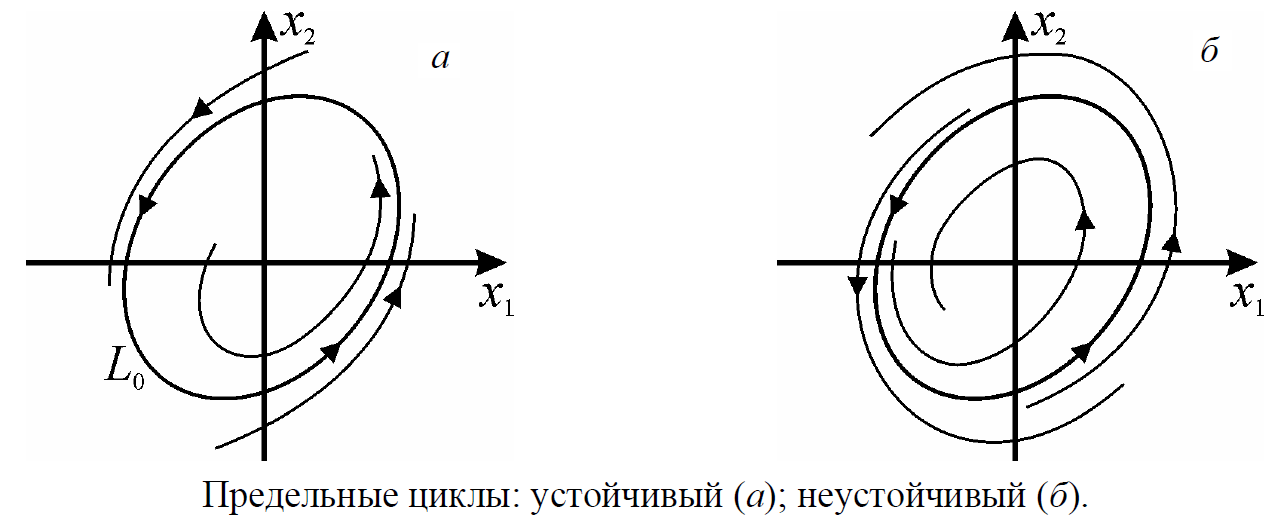
\includegraphics[width=0.7\linewidth]{tk_img/predel.png}\\
		\textbf{Характеристики:}\\
		$\divideontimes$ Мультипликатор $S$: $S<1$ - ПЦ устойчивый, $S>1$ - ПЦ неустойчивый. Всегда $S>0$\\
		$\divideontimes$ Характерестический показатель $\lambda$: $\lambda<0$ - ПЦ устойчивый, $\lambda>0$ - ПЦ неустойчивый. $\lambda$ можем получить в уравнении при линеаризации системы\\
		Связь характеристик: $\lambda = \dfrac{1}{T_0}ln(S)$
		
		\section{Автоколебания и автоколебательная система. Мягкий и жесткий режимы возбуждения}
		Автоколебательная система — диссипативная система, совершающая незатухающие колебания при отсутствии колебательного воздействия извне. В этих системах возникает баланс между действиями диссипативных потерь и внутренних механизмов, компенсирующих потери. Автоколебания — незатухающие колебания в нелинейной диссипативной системе, форма и свойства которых в определенных пределах не зависит от начальных условий и определяется параметрами самой системы.\\
		\textbf{1. Мягкий режим\\}
		$\gamma < 0$ - автоколебаний нет, $\gamma = 0$ - суперкритическая бифуркация Андронова-Хопфа ($\lambda_i < 0$), $\gamma > 0$ - неустойчивое состояние равновесия + появление одного устойчивого предельного цикла на фазовой плоскости. \quad $\gamma \uparrow A \uparrow$\\\\
		Состояние равновесия $\gamma = 0$ - безопасная граница устойчивости, то есть при ее нарушении система переходят в качественно новое состояние, но не покидает при $0<\gamma \ll 1$ окрестности предыдущего состояния.\\
		\textbf{2. Жесткий режим\\}
		$\lambda< 0$ - состояние равновесия локально устойчиво, $\lambda = 0$ - состояние равновесия теряет устойчивость $\rightarrow$ автоколебания возникают скачком (жестко), $\lambda \uparrow A \uparrow$, затем квазистатически $\lambda \downarrow A \uparrow$ от $\lambda > 0$, а потом совсем исчезают скачком. Рождение и исчезновение АК происходит при разных $\lambda$ - наблюдается гестерезис. $\lambda = 0$ - опасная граница устойчивости состояния равновесия, так как поведение системы менятеся резко\\
		\begin{tabular}{c c}
			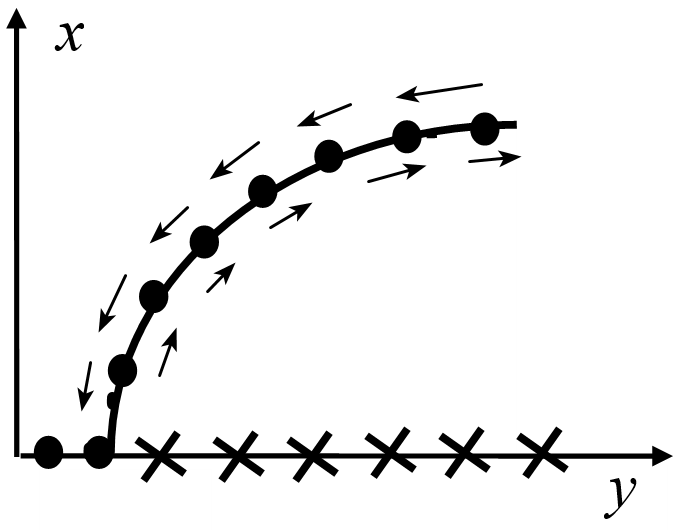
\includegraphics[width=0.40\linewidth]{tk_img/avtokoleb_1.png} & 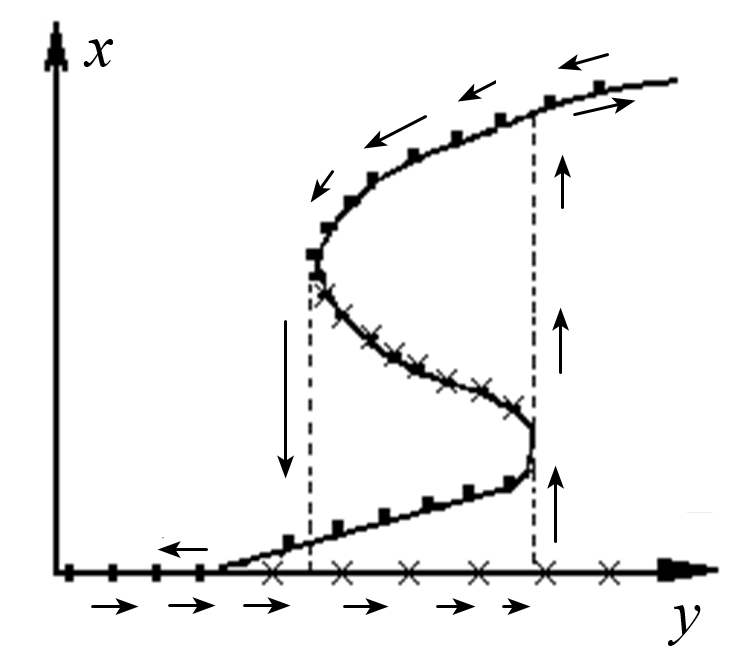
\includegraphics[width=0.35\linewidth]{tk_img/avtokoleb_2.png}
		\end{tabular}\\
		
		\textbf{Свойства автоколебательных систем}\\
		$\divideontimes$ Источник энергии для компенсации диссипации — постоянен и находится внутри самой системы\\
		$\divideontimes$ Система содержит колебательную подсистему и активный нелинейный элемент\\
		$\divideontimes$ В изолированной колебательной системе происходят затухающие колебательные процессы, а активный элемент может усиливать колебания и их нелинейно ограничивать\\
		$\divideontimes$ Между колебательной подсистемой активным элементом существует обратная связь, регулирующая поступление энергии от источника\\
		$\divideontimes$ Автоколебания в определенных пределах не зависят от начальных условиях и определяются параметрами системы\\
		$\divideontimes$ Математическим образом периодических автоколебаний является предельной цикл
		
		\section{Бифуркационные сценарии рождения периодических движений динамических систем на плоскости}
		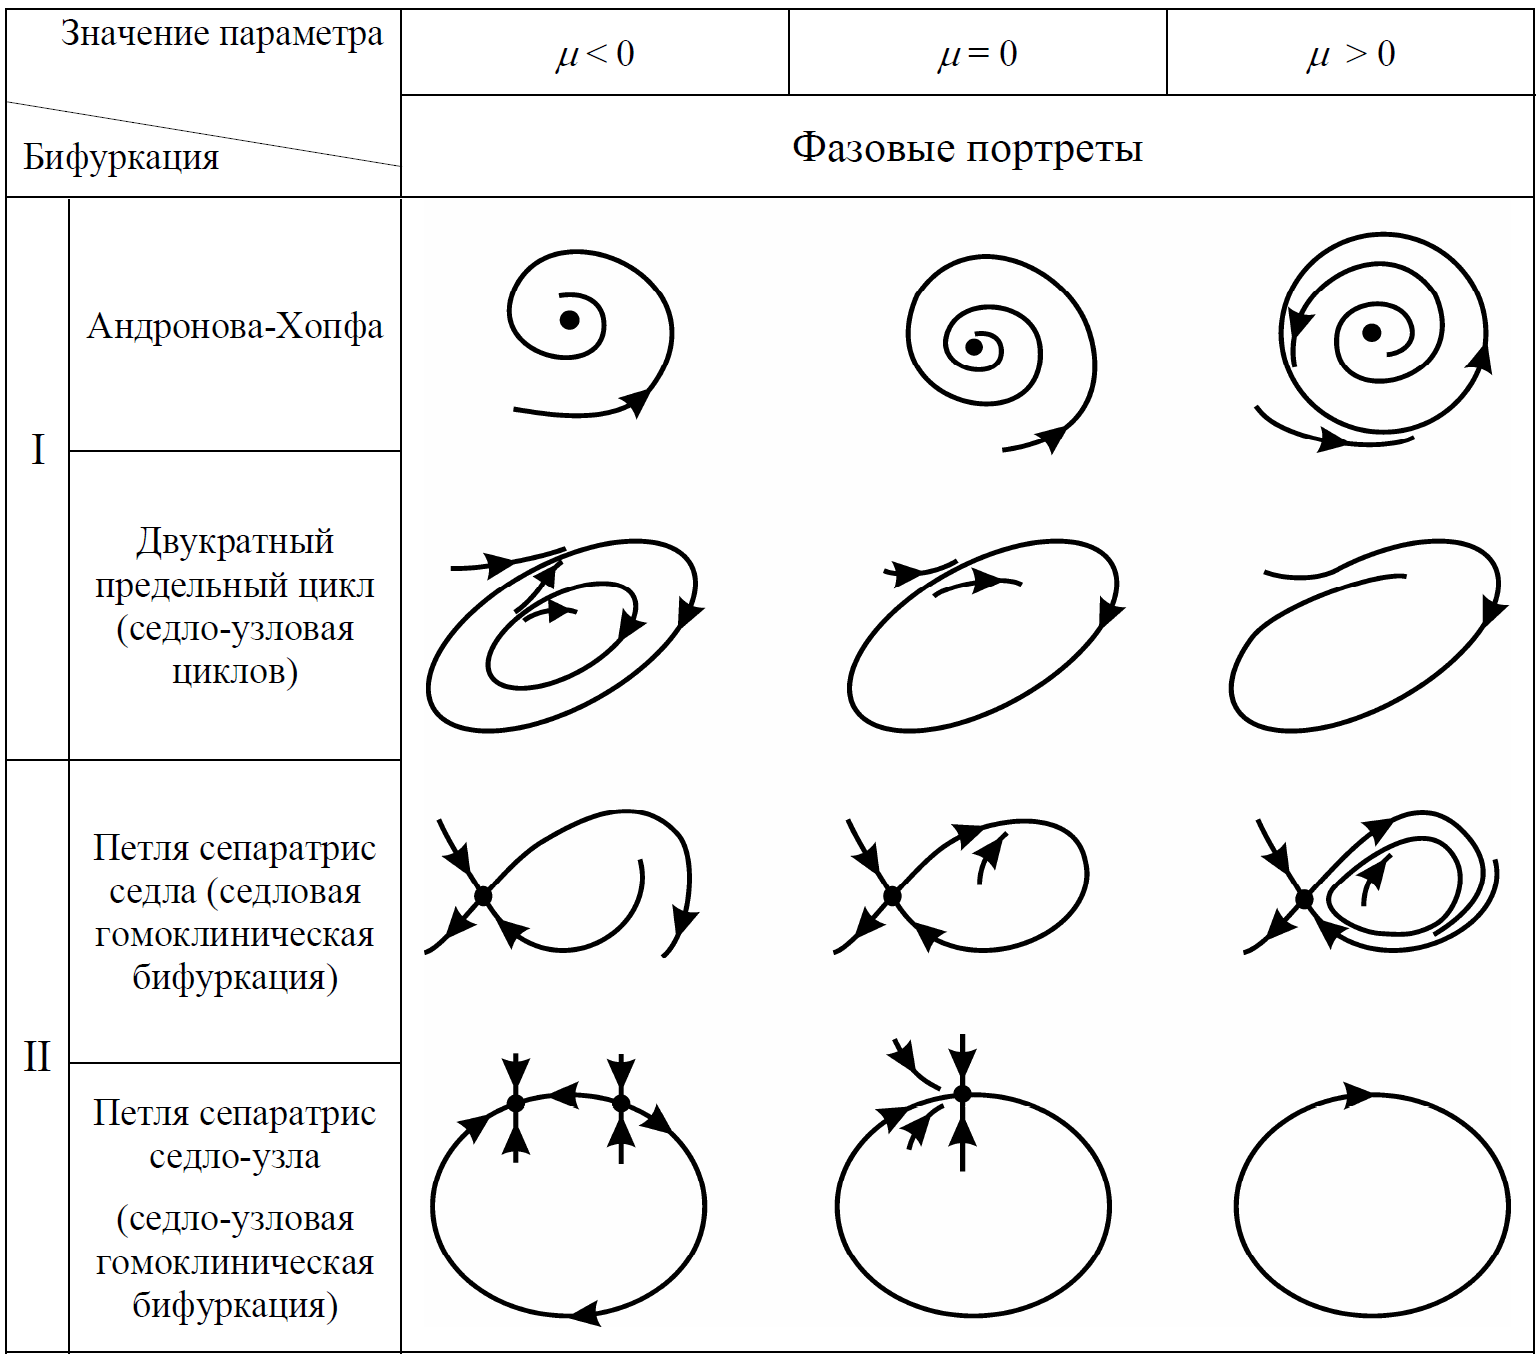
\includegraphics[width=0.75\linewidth]{tk_img/bifurk.png}
		
		\section{Дисперсия, ее физическая природа и проявления}
		Дисперсия — зависимость фазовой скорости волны от ее частоты. Связь между частотой и волновым числом гармонической волны определяется пространственными и временными масштабами среды и называется дисперсионным соотношением.
		
		\begin{tabular}{c c}
			\begin{tabular}{c}
				$\omega^2 = \omega_0^2 + \dfrac{4\gamma }{m}sin^2(\dfrac{ka}{A})$\\
				$a$ - расстояние между маятниками\\
				$\gamma$ - жесткость пружины\\
				$k$ - действительное волновое число	\\ 
				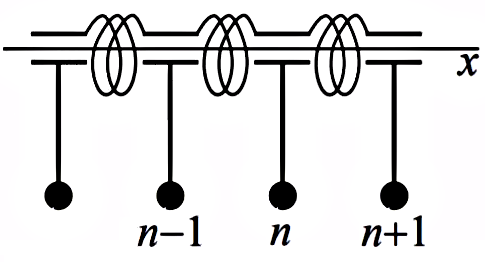
\includegraphics[width=0.4\linewidth]{tk_img/dispers_2.png}\\
			\end{tabular} & \begin{tabular}{c}
				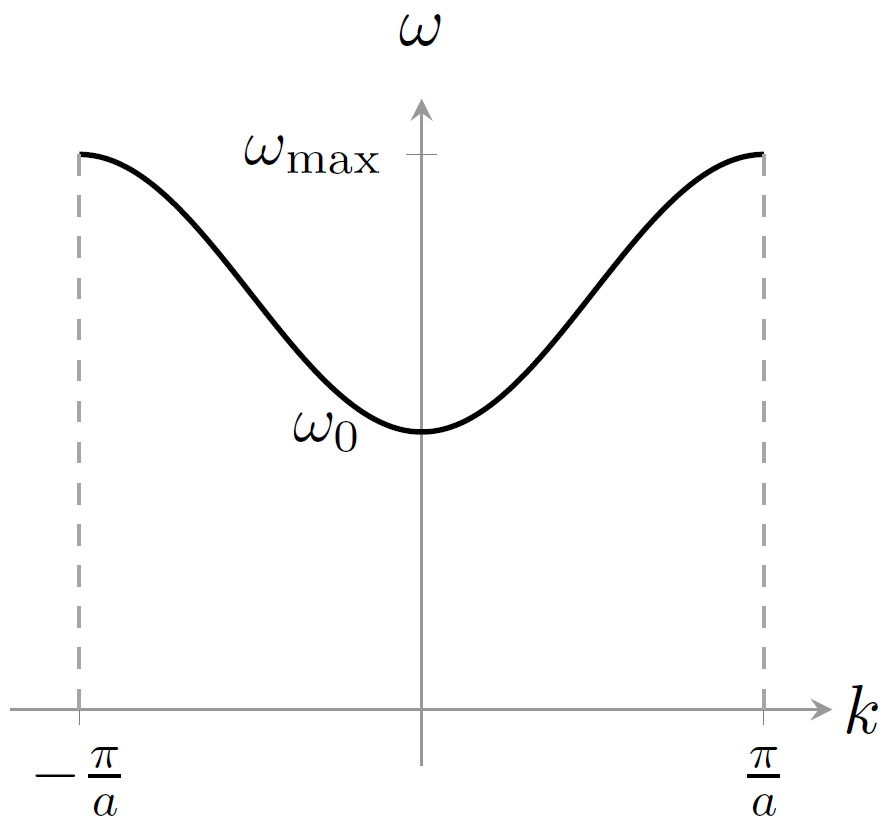
\includegraphics[width=0.35\linewidth]{tk_img/dispers.png}\\
			\end{tabular}
		\end{tabular}\\
		У каждой компоненты волнового пакета будет своя $V_\text{ф}$, возникает его деформация. Наличием собственных масштабов объясняется эффект частичного непропускания волны\\
		Область прозрачности: $k\in Re$ - распространение без искажения гармонической волны\\
		Область непрозрачности: $k\in Im$ - нераспространение.
		
		\section{Простые волны. Основные свойства и условия существования}
		$U_t + C(U)U_x = 0$ — нелинейное уравнение простой волны. $C(U)$ — дифференцируемая функция (скорость от состояния среды). Характеристики — линии, вдоль которых переменная $U(x, t)$ будет оставаться постоянной и равной по значению для каждого соответствующего значения $x$.\\
		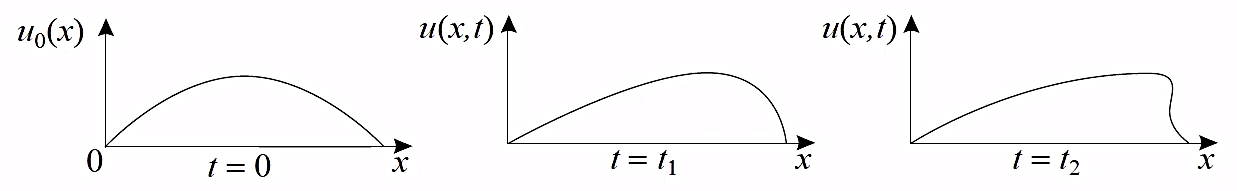
\includegraphics[width=1\linewidth]{tk_img/prost_voln_1.png}\\
		\begin{tabular}{l c}
			\begin{tabular}{l}
				В точке пересечения \\характеристик их значения\\ одинаковы — появится точка\\ разрыва (производная равна $\infty$)\\ - градиентная катастрофа.\\ На переднем фронте образуется \\ударная волна. Уравнение перестает \\работать после точки разрыва.
			\end{tabular} & \begin{tabular}{c}
				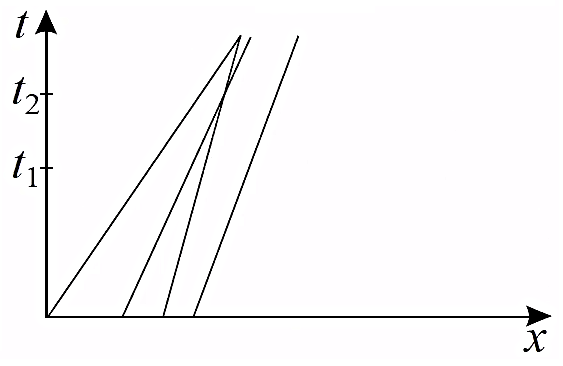
\includegraphics[width=0.35\linewidth]{tk_img/prost_voln_2.png}\\
			\end{tabular}
		\end{tabular}
		
		\section{Параметрические системы. Основные свойства}
		Параметрически системы — системы, где внешнее воздействие находится внутри системы и может изменять ее параметры.\\
		\textbf{Резонансные. } Период изменения параметров находится в целочисленном соотношении с периодом собственных колебаний. В такт с изменением энергии, соответствующей собственным колебаниям, вносится энергия, вызванная работой внешнего воздействия. При определенных условиях может привести к эффекту раскачки колебаний за счет накапливающейся в системе энергии. \\
		\textbf{Нерезонансные. }Параметры изменяются очень быстро или очень медленно в сравнении с характерными временными масштабами изменения переменных системы.\\
		\textbf{Свойства.}\\
		1. Параметрическая система, находящаяся в начальный момент в состоянии равновесия, останется в этом состоянии при $t>0$ (дергая за нитку, маятник нельзя раскачать)\\
		2. Состояния равновесия параметрической системы могут быть как устойчивы, так и неустойчивы\\
		3. Если параметры системы таковы, что она неустойчива и система выведена из состояния равновесия, то в ней возникают колебания, амплитуда которых $\uparrow exp$. Процесс возрастания размаха в колебаний при периодическом нарастании колебаний — параметрический резонанс.
		
		\section{Релаксационные колебания}
		
		\section{Локальные бифуркации состояний равновесия трехмерных систем}
		
		\section{Локальные бифуркации периодических движений трехмерных систем}
		
	\end{multicols*}
\end{document}
